\documentclass[11pt]{beamer}
\usepackage[T1]{fontenc}
\usepackage{lmodern}
\usepackage[]{import}
\usepackage[]{graphicx}
\usepackage[export]{adjustbox}
\usepackage{lmodern}
\usepackage[]{minted}
\setminted{linenos=true, numbersep=5pt, xleftmargin=20pt}
\makeatletter
\AtBeginEnvironment{minted}{\dontdofcolorbox}
\def\dontdofcolorbox{\renewcommand\fcolorbox[4][]{##4}}
\makeatother
\usetheme{Boadilla}


\begin{document}
	\author{Maël Petit n°32502}
	\title{JEU D'ECHECS QUANTIQUES}
	\subtitle{}
	%\logo{}
	%\institute{}
	\date{}
	%\subject{}
	%\setbeamercovered{transparent}
	%\setbeamertemplate{navigation symbols}{}
	\begin{frame}[plain]
		
		\maketitle
		
\includegraphics[scale = 0.15, center]{./intro-presentation.jpg} 

	\end{frame}
	
	\begin{frame}
		
		\frametitle{Présentation des règles du jeu}
		$\bullet$ 2 joueurs qui jouent à tour de rôle \newline
		$\bullet$ Sur un carré plateau de 64 cases \newline
		$\bullet$ Différents types de pièces \newline
		$\bullet$ Un tour = un mouvement \newline %mal dit
		$\bullet$ Objectif : capturer le roi adverse \newline     

	\end{frame}
	
	\begin{frame}
		\frametitle{Mouvements classique}
		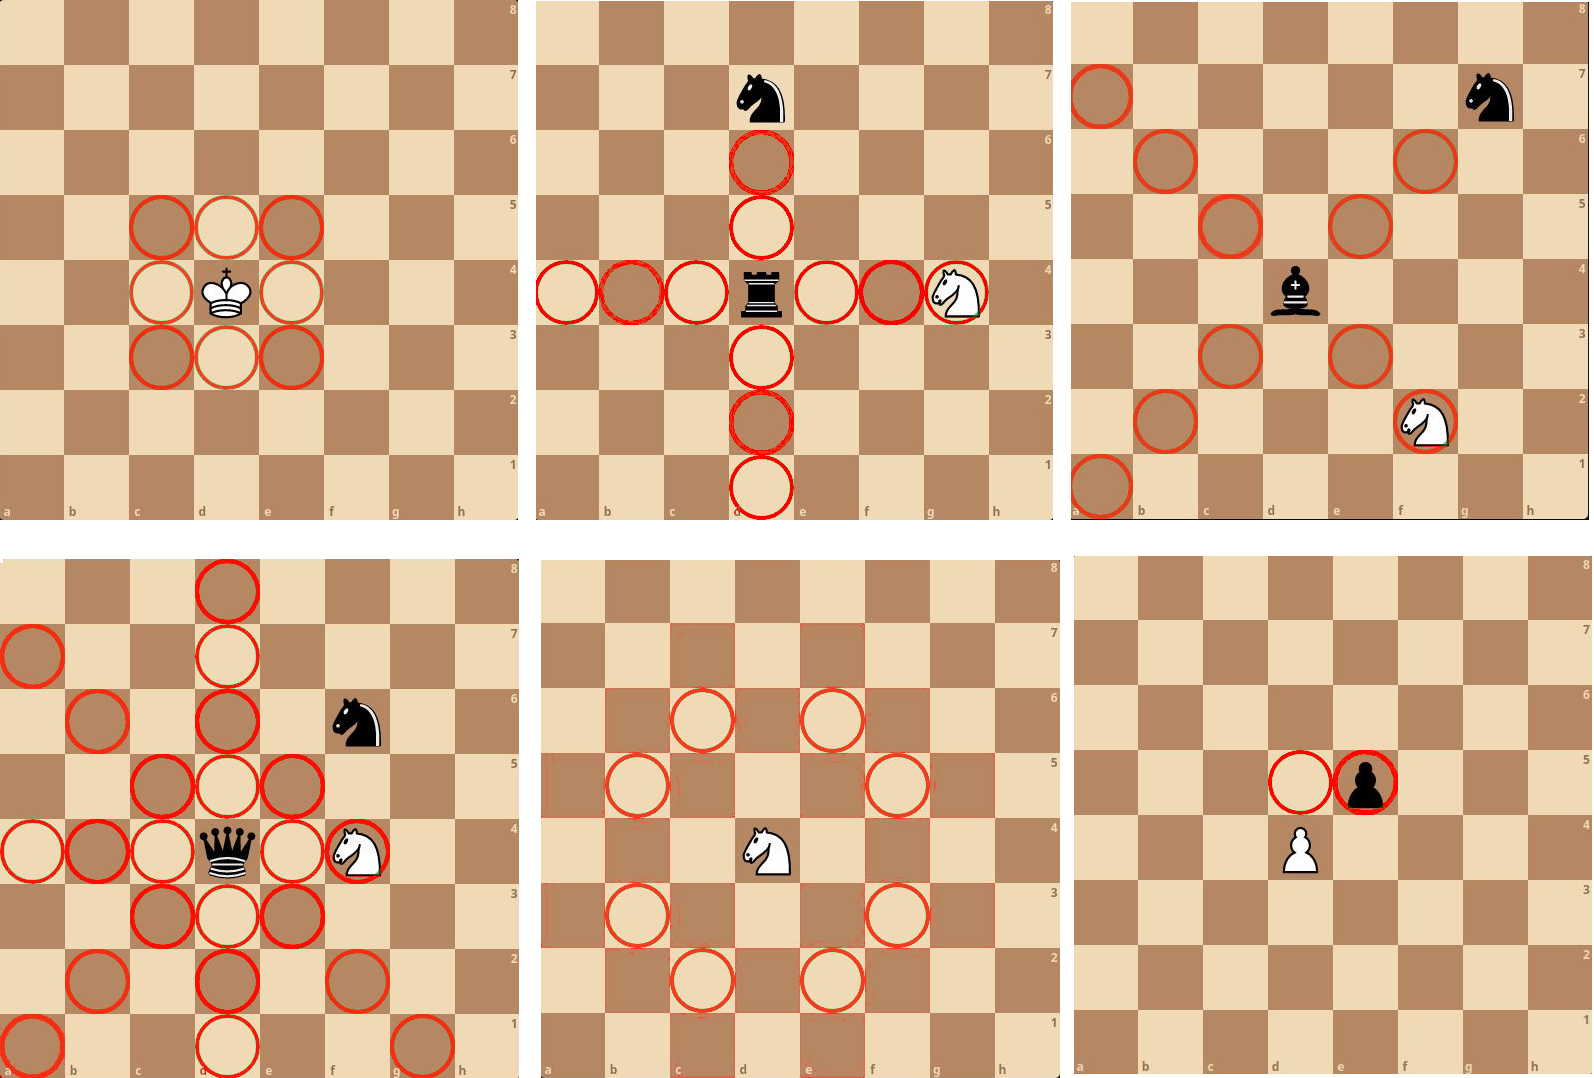
\includegraphics[scale = 0.9, center]{./classic-chess.png}    

	\end{frame}
	
	\begin{frame}
		\frametitle{Mouvement split}
		% Aucun des deux joueurs n'a l'information
		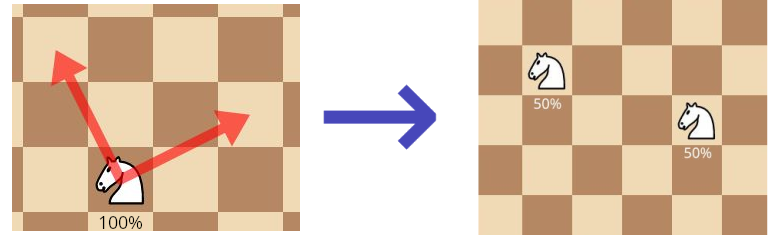
\includegraphics[scale = 0.45, center]{./split.png}    
	%	{\tiny lichess.org}

	\end{frame}
	
	\begin{frame}
		
		\frametitle{Mouvement merge}
		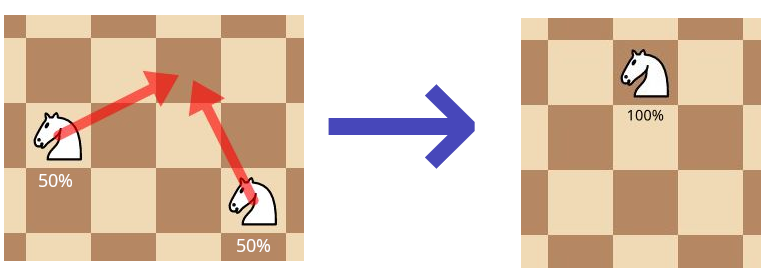
\includegraphics[scale = 1.7, center]{./merge.png}    

	\end{frame}
	
	\begin{frame}
		
		\frametitle{Principe des mesures}
		%$\bullet$ Non-occupation simultanée 
		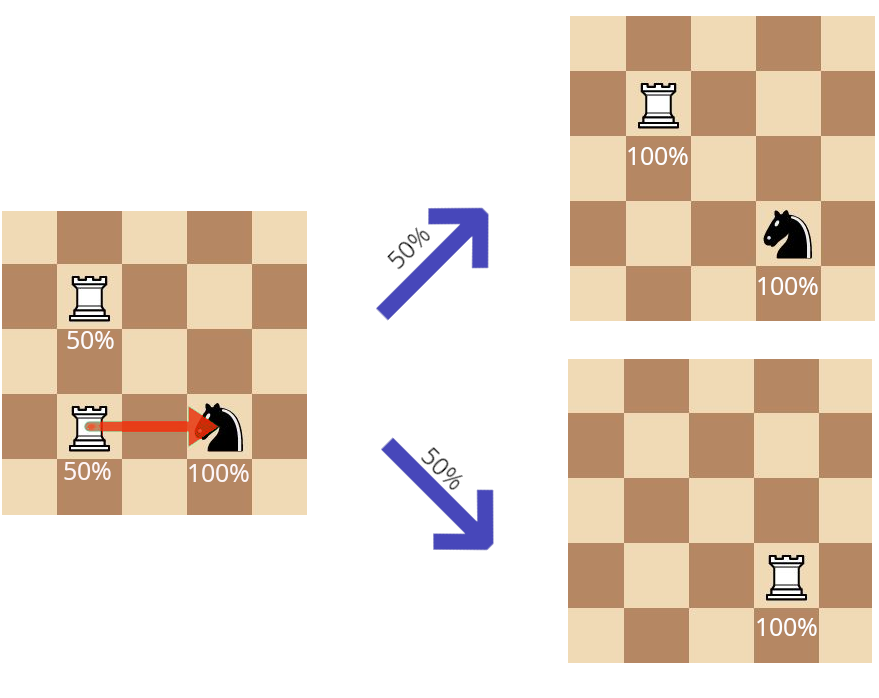
\includegraphics[scale = 1.4, center]{./mesure.png}    
	
\end{frame}
	
	\begin{frame}
		
		\frametitle{Objectif : Etude de la finale fou-cavalier contre dame}
		$\bullet$ Diminution de la taille du plateau \newline
		$\bullet$ Jeu d'échecs classique : finale gagnate pour les blancs mais difficile à gagner \newline
		$\bullet$ Jeu d'échecs quantique : stratégie simple pour avoir une chance de gagner rapidement 
		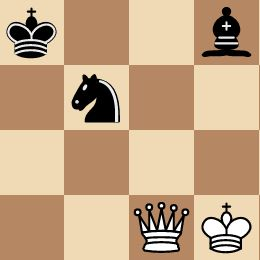
\includegraphics[scale = 1, center]{./pos1_exp1.jpg}	

	\end{frame}
	
	\begin{frame}
		
		\frametitle{Algorithme min-max : principe}
		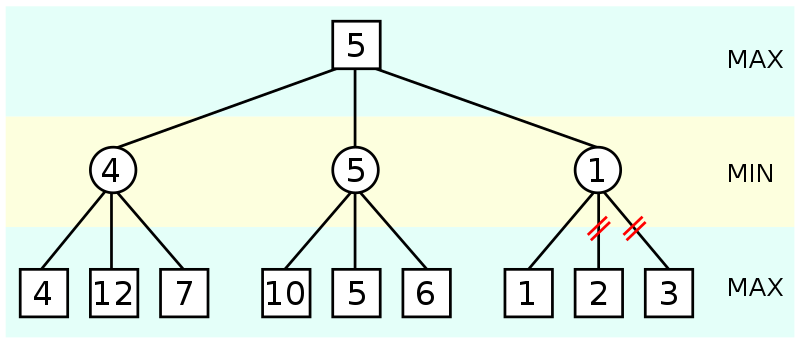
\includegraphics[scale=1, center]{alpha-beta.png} \newline
		
			\end{frame}
	
	\begin{frame}
		
		\frametitle{Elagage alpha-beta : principe}
		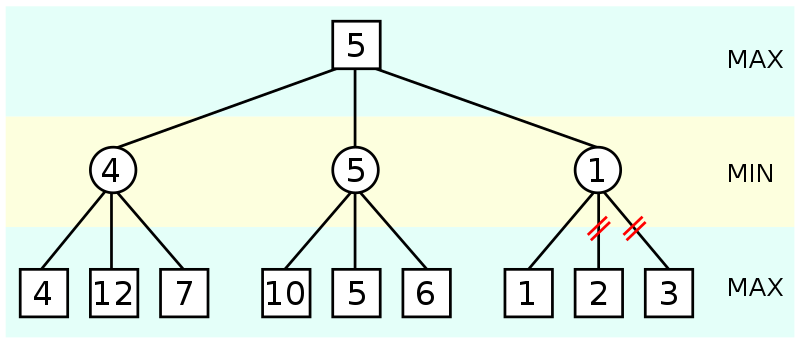
\includegraphics[scale=1, center]{alpha-beta.png} \newline
		
			\end{frame}
	\begin{frame}
		\frametitle{Algorithme min-max}
		$\bullet$ Besoin d'être adapté lors des mesures\newline 
		$\bullet$ Fonction d'évaluation des noeuds : \newline
		\begin{equation}
			\notag
			eval(\mathcal{B}) =
			\begin{cases}
				\ \; 1 & \mathcal{B} \text{ est gagnant pour le joueur blanc}\\
				-1 & \mathcal{B} \text{ est gagnant pour le joueur noir } \\
				0 & \text{ sinon}
			\end{cases}       
		\end{equation}
		$\bullet$ Calcul de la valeur d'un mouvement : \newline
		$proba_1*board_1 + proba_2*board_2$ \newline
		$\bullet$ Pas d'élagage alpha-béta après une mesure
	\end{frame}
	
	\begin{frame}
		\frametitle{Résolution su un exemple}
		$\bullet$ Profondeur = 4
		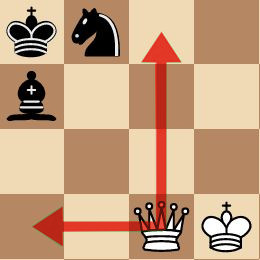
\includegraphics[scale = 1, center]{./pos2_exp1.jpg}	
	\end{frame}
	
	\begin{frame}
		\frametitle{Résolution sur un exemple}
	%	$\bullet$ Profondeur = 4
		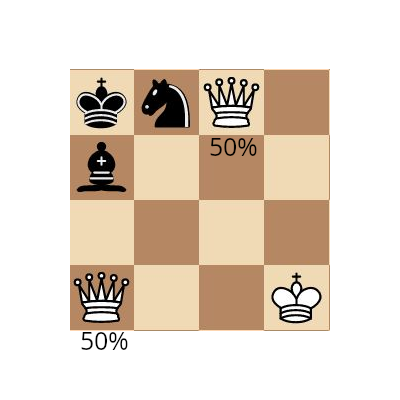
\includegraphics[scale = 1, center]{./pos3_exp1.png}	
	
\end{frame}
	
	\begin{frame}
		\frametitle{Résolution sur un exemple}
	%	$\bullet$ Profondeur = 4
		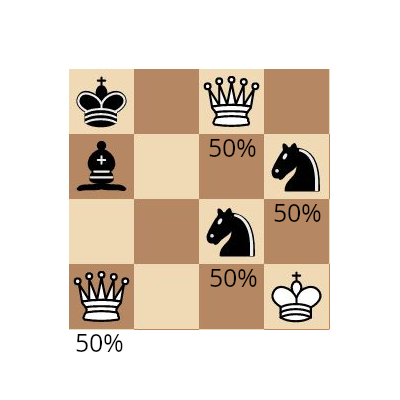
\includegraphics[scale = 1, center]{./pos4_exp1.png}	
	\end{frame}

	\begin{frame}
		\frametitle{Résolution sur un exemple}
	%	$\bullet$ Profondeur = 4
		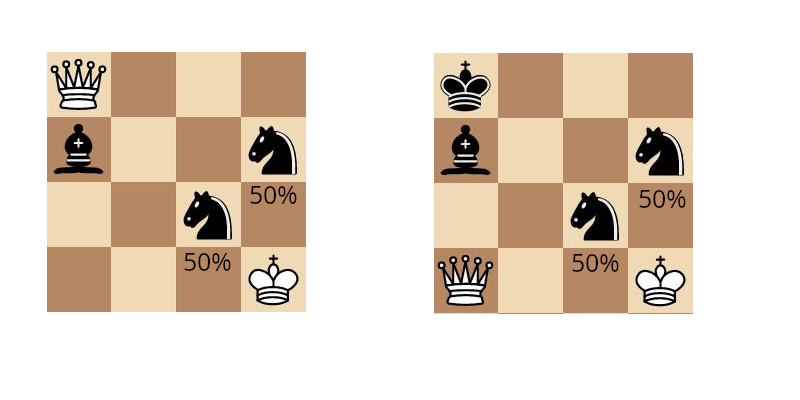
\includegraphics[scale = 1.5, center]{./pos5_exp1.png}	
	\end{frame}

	\begin{frame}
		\frametitle{Effet horizon}
	%	$\bullet$ La finale suivante est gagnante pour les noirs
		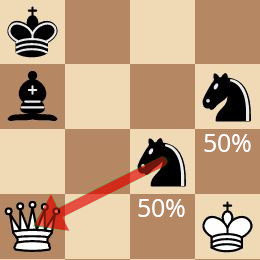
\includegraphics[scale = 0.5, center]{./hor1.png}	
		$\bullet$ Changement de la fonction d'évaluation : \newline
		\begin{equation}
			\notag
			eval(\mathcal{B}) =
			\begin{cases}
				\ \; 1 & \mathcal{B} \text{ est gagnant pour le joueur blanc}\\
				-1 & \mathcal{B} \text{ est gagnant pour le joueur noir } \\
				-P & \text{ si la dame blanche est capturée et que le joueur noir a} \\ 
					& \text{ encore son cavlier et son fou} \\
				0 & \text{ sinon}
			\end{cases}       
		\end{equation}
		$\bullet$ Cette fonction d'évaluation semble favoriser les noirs

	\end{frame}

\begin{frame}
	
	\frametitle{Test sur des exemples générés aléatoirement}
	$\bullet $ Les pièces sont positionnées aléatoirement \newline
	$\bullet $ Le joueur blanc joue en premier \newline
	$\bullet $ Profondeur = 4
	\begin{center}
		
		\begin{tabular}{ | l | c | }
			\hline
			Nombre de plateaux passés & 722 \\ \hline
			Moyenne & 0.08 \\ \hline
			$-1 < val < -0.75$ & 5  \\ \hline
			$-0.75 < val < -0.5$ & 0  \\ \hline
			$-0.5 < val < -0.25$ & 2  \\ \hline
			$-0.25 < val < 0$ & 0 \\ \hline
			$val = 0 $   & 239  \\ \hline
			$0 < val < 0.25$ & 1  \\ \hline
			$0.25 < val < 0.5$ & 4  \\ \hline
			$0.5 < val < 0.75$ & 0  \\ \hline
			$0.75 < val < 1$ & 27  \\
			\hline
		\end{tabular}
	\end{center}	
\end{frame}

\begin{frame}
	\frametitle{Test sur des exemples générés aléatoirement}
	$\bullet $ Les pièces sont positionnées aléatoirement, sauf les rois qui sont placés sur des bords opposés \newline
	$\bullet $ Le joueur blanc joue en premier \newline
	$\bullet $ Profondeur = 4
	\begin{center}
		
		\begin{tabular}{ | l | c | }
			\hline
			Nombre de plateaux passés & 524 \\ \hline
			Moyenne & 0.01 \\ \hline
			$-1 < val < -0.75$ & 1  \\ \hline
			$-0.75 < val < -0.5$ & 0  \\ \hline
			$-0.5 < val < -0.25$ & 1  \\ \hline
			$-0.25 < val < 0$ & 0 \\ \hline
			$val = 0 $   & 458  \\ \hline
			$0 < val < 0.25$ & 4  \\ \hline
			$0.25 < val < 0.5$ & 9  \\ \hline
			$0.5 < val < 0.75$ & 0  \\ \hline
			$0.75 < val < 1$ & 3  \\
			\hline
			\hline
		\end{tabular}
	\end{center}	
\end{frame}

\begin{frame}
	\frametitle{Test sur des exemples générés aléatoirement}
	$\bullet $ Les pièces sont positionnées aléatoirement, sauf les rois qui sont placés sur des bords opposés \newline
	$\bullet $ Le joueur noir joue en premier \newline
	$\bullet $ Profondeur = 4
	\begin{center}
		\begin{tabular}{ | l | c | }
			\hline
			Nombre de plateaux passés & 743 \\ \hline
			Moyenne & 0.00 \\ \hline
			$-1 < val < -0.75$ & 0  \\ \hline
			$-0.75 < val < -0.5$ & 0  \\ \hline
			$-0.5 < val < -0.25$ & 0  \\ \hline
			$-0.25 < val < 0$ & 0 \\ \hline
			$val = 0 $   & 256  \\ \hline
			$0 < val < 0.25$ & 0  \\ \hline
			$0.25 < val < 0.5$ & 0  \\ \hline
			$0.5 < val < 0.75$ & 0  \\ \hline
			$0.75 < val < 1$ & 1  \\
			\hline
		\end{tabular}
	\end{center}
\end{frame}

	\begin{frame}
	\frametitle{Conclusion}
	$\bullet$ Les mouvement quantiques favorisent l'attaque \newline
	$\bullet$ Le joueur qui a le trait est avantagé comme au jeu d'échecs classique \newline
	$\bullet$ Profondeur faible \newline
	$\bullet$ L'effet horizon empêche d'avoir des résultats précis \newline
	
\end{frame}
	%\import{./../}{code-latex-output}      

\end{document}